\documentclass[12pt,a4paper]{article}
\usepackage[utf8]{inputenc}
\usepackage[spanish]{babel}
\usepackage{amsmath}
\usepackage{amsfonts}
\usepackage{amssymb}
\usepackage{graphicx}
\usepackage{geometry}
\usepackage{booktabs}
\usepackage{array}
\usepackage{multirow}
\usepackage{float}
\usepackage{subcaption}
\usepackage{listings}
\usepackage{xcolor}
\usepackage{hyperref}

% Configuración para listings (código Python)
\lstset{
    language=Python,
    basicstyle=\ttfamily\footnotesize,
    keywordstyle=\color{blue}\bfseries,
    commentstyle=\color{green!60!black},
    stringstyle=\color{red},
    numbers=left,
    numberstyle=\tiny\color{gray},
    stepnumber=1,
    numbersep=5pt,
    showspaces=false,
    showstringspaces=false,
    showtabs=false,
    frame=single,
    tabsize=4,
    captionpos=b,
    breaklines=true,
    breakatwhitespace=false,
    backgroundcolor=\color{gray!10}
}

\geometry{margin=2.5cm}

\title{\textbf{Examen: Statistical Learning}}
\author{Andrés Proaño}
\date{\today}

\begin{document}

\maketitle

\section{Ejercicio 1: Boston Housing Datasets}

Se trabajará con el dataset Boston Housing que contiene información sobre viviendas en Boston, Massachusetts. El objetivo es predecir el valor mediano de las viviendas.

El dataset contiene las siguientes variables:
\begin{itemize}
\item CRIM     per capita crime rate by town
\item ZN       proportion of residential land zoned for lots over 25,000 sq. ft.
\item INDUS    proportion of non-retail business acres per town
\item CHAS     Charles River dummy variable (1 if tract bounds river; 0 otherwise)
\item  AGE      proportion of owner-occupied units built prior to 1940
\item  DIS      weighted distances to five Boston employment centres
\item  RAD      index of accessibility to radial highways
\item  TAX      full-value property-tax rate per \$10,000
\item  PTRATIO  pupil-teacher ratio by town
\item  B        1000(Bk - 0.63)^2 where Bk is the proportion of blacks by town
\item  LSTAT    porcentaje de población de bajo estatus
\item  MEDV     Median value of owner-occupied homes in \$1000's
\end{itemize}

\subsection{Base de Datos}

Se utilizó el conjunto de datos Boston Housing disponible en la Universidad de Toronto con fines educativos.

\begin{lstlisting}[language=Python, frame=single, basicstyle=\ttfamily\small, breaklines=true]
data_url = "http://lib.stat.cmu.edu/datasets/boston"
raw_df = pd.read_csv(data_url, sep="\s+", skiprows=22, header=None)
data = np.hstack([raw_df.values[::2, :], raw_df.values[1::2, :2]])
target = raw_df.values[1::2, 2]
\end{lstlisting}

\subsection{Objetivo}

El objetivo es predecir el valor mediano de las viviendas comparando diferentes modelos y sus rendimientos.

\subsection{Tareas Requeridas}

\subsubsection{Implementación de Modelos}

Antes de realizar los diferentes modelos, vamos a buscar significancia dentro de las variables para evitar utilizar datos que no aporten al trabajo.

\begin{figure}[H]
\centering
% Primera fila
\begin{subfigure}[t]{0.24\textwidth}
    \centering
    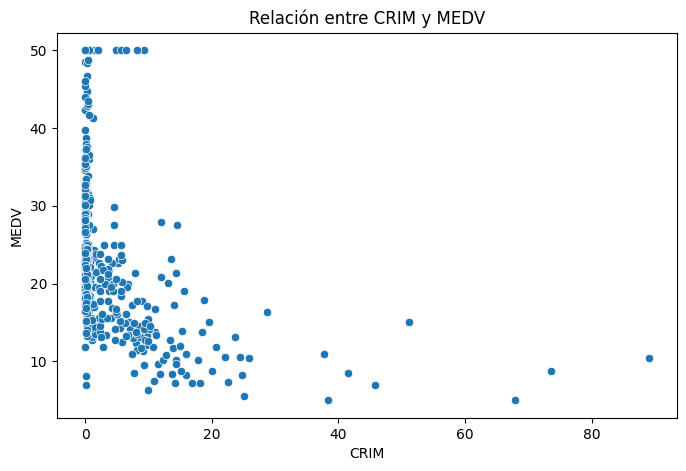
\includegraphics[width=\textwidth]{figures/crim_medv.png}
    \caption{\footnotesize Tasa de criminalidad per cápita}
    \label{fig:modelo_crim}
\end{subfigure}
\hfill
\begin{subfigure}[t]{0.24\textwidth}
    \centering
    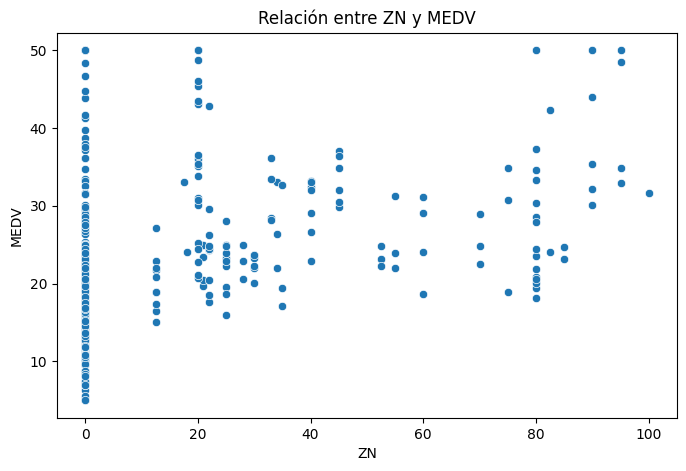
\includegraphics[width=\textwidth]{figures/zn_medv.png}
    \caption{\footnotesize Proporción de terrenos residenciales}
    \label{fig:modelo_zn}
\end{subfigure}
\hfill
\begin{subfigure}[t]{0.24\textwidth}
    \centering
    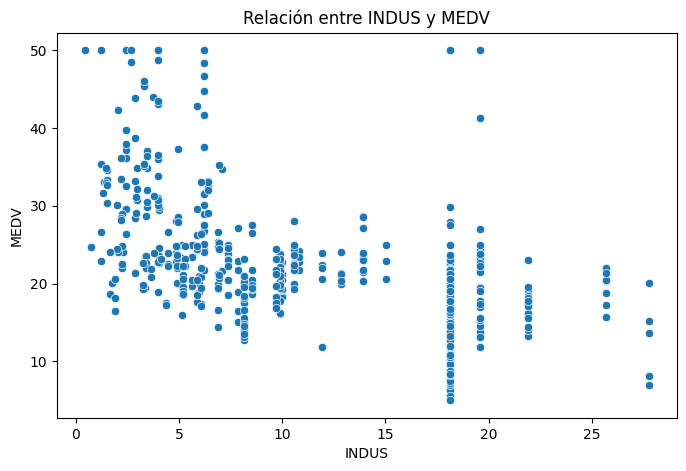
\includegraphics[width=\textwidth]{figures/indus_medv.png}
    \caption{\footnotesize Proporción de terrenos industriales}
    \label{fig:modelo_indus}
\end{subfigure}
\hfill
\begin{subfigure}[t]{0.24\textwidth}
    \centering
    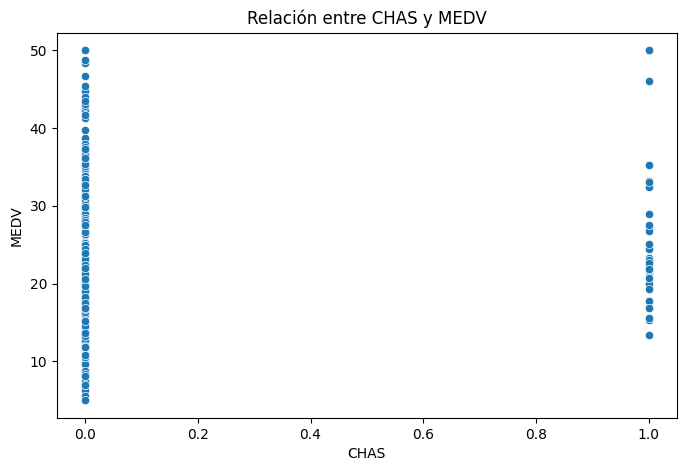
\includegraphics[width=\textwidth]{figures/chas_medv.png}
    \caption{\footnotesize Variable Dummy del Río Charles}
    \label{fig:modelo_chas}
\end{subfigure}

\vspace{0.2cm}

% Segunda fila
\begin{subfigure}[t]{0.24\textwidth}
    \centering
    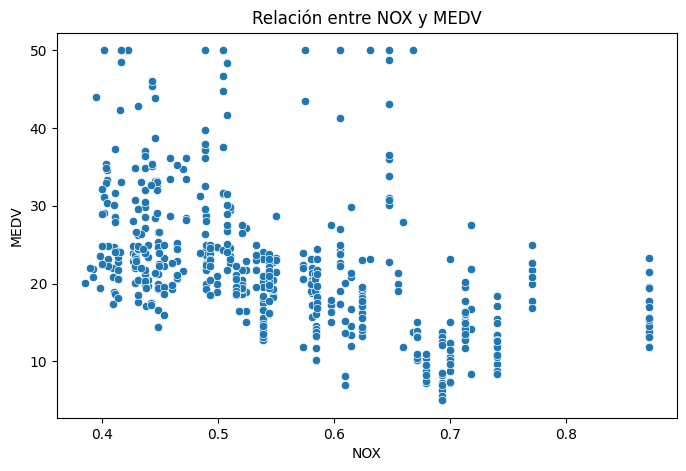
\includegraphics[width=\textwidth]{figures/nox_medv.png}
    \caption{\footnotesize Concentración de Óxidos de Nitrógeno}
    \label{fig:modelo_nox}
\end{subfigure}
\hfill
\begin{subfigure}[t]{0.24\textwidth}
    \centering
    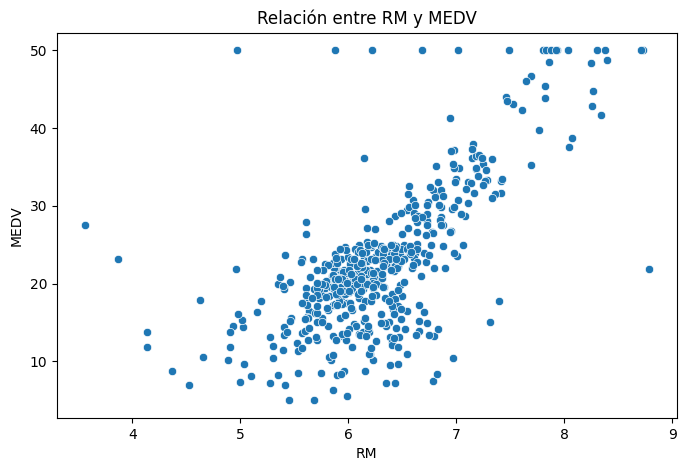
\includegraphics[width=\textwidth]{figures/rm_medv.png}
    \caption{\footnotesize Número promedio de habitaciones}
    \label{fig:modelo_rm}
\end{subfigure}
\hfill
\begin{subfigure}[t]{0.24\textwidth}
    \centering
    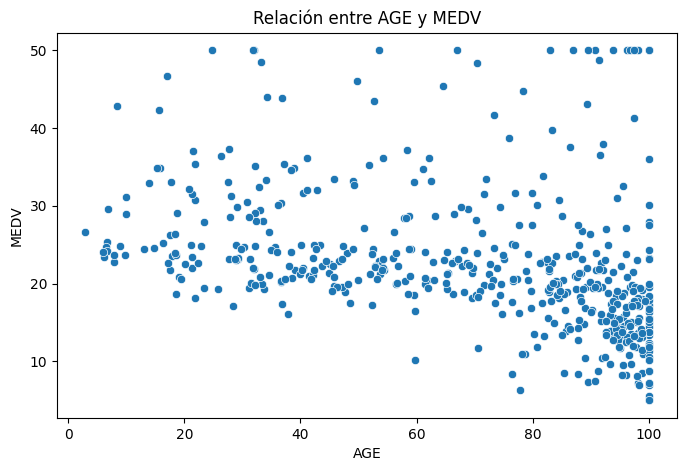
\includegraphics[width=\textwidth]{figures/age_medv.png}
    \caption{\footnotesize Edad}
    \label{fig:modelo_age}
\end{subfigure}
\hfill
\begin{subfigure}[t]{0.24\textwidth}
    \centering
    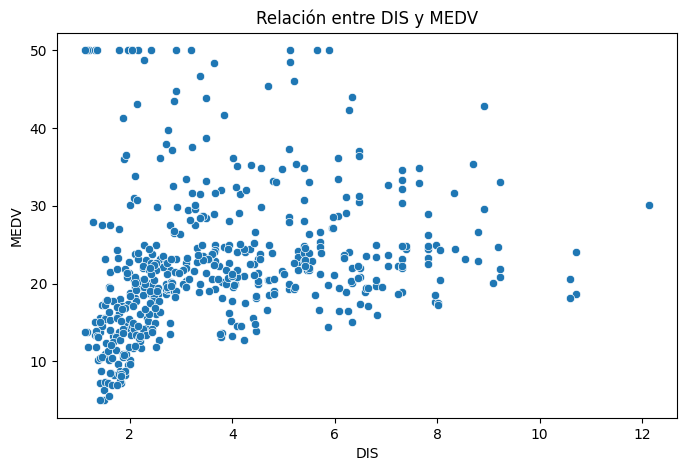
\includegraphics[width=\textwidth]{figures/dis_medv.png}
    \caption{\footnotesize Distancia a centros de empleo}
    \label{fig:modelo_dis}
\end{subfigure}

\vspace{0.2cm}

\begin{subfigure}[t]{0.24\textwidth}
    \centering
    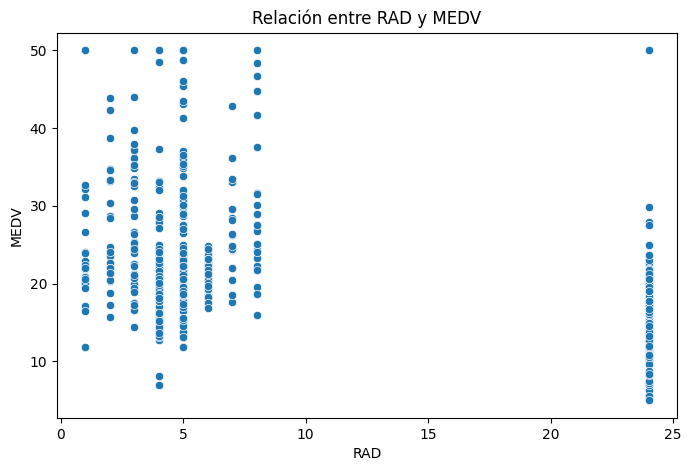
\includegraphics[width=\textwidth]{figures/rad_medv.png}
    \caption{\footnotesize Accesibilidad a autopistas radiales}
    \label{fig:modelo_rad}
\end{subfigure}
\hfill
\begin{subfigure}[t]{0.24\textwidth}
    \centering
    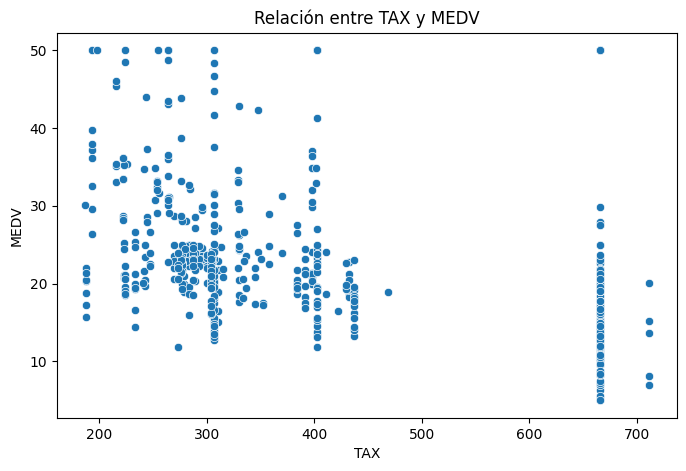
\includegraphics[width=\textwidth]{figures/tax_medv.png}
    \caption{\footnotesize Tasa de impuesto predial}
    \label{fig:modelo_tax}
\end{subfigure}
\hfill
\begin{subfigure}[t]{0.24\textwidth}
    \centering
    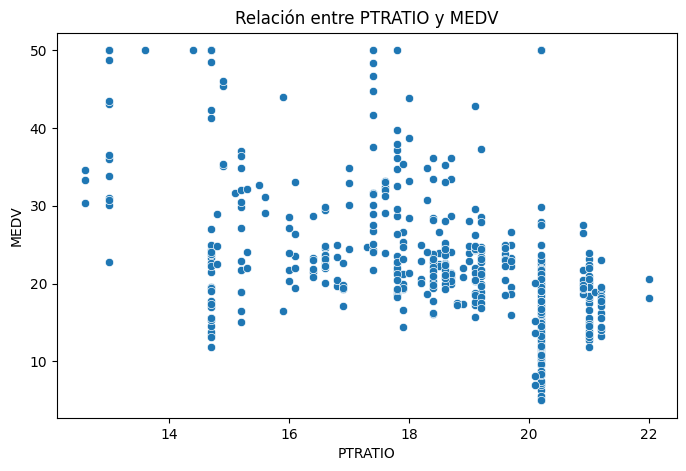
\includegraphics[width=\textwidth]{figures/ptratio_medv.png}
    \caption{\footnotesize Relación de Población por Área}
    \label{fig:modelo_ptratio}
\end{subfigure}
\hfill
\begin{subfigure}[t]{0.24\textwidth}
    \centering
    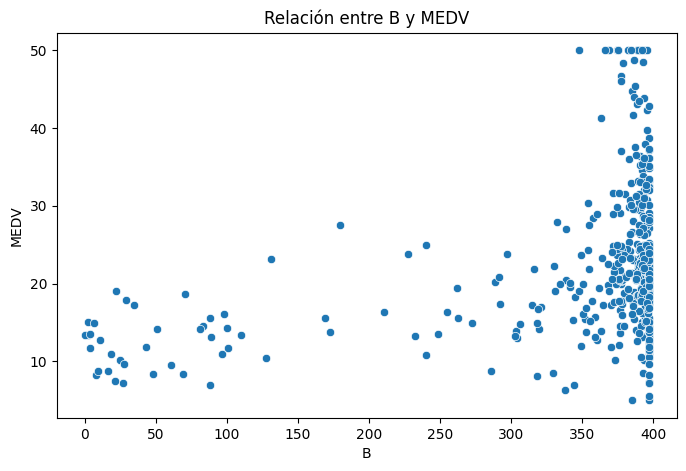
\includegraphics[width=\textwidth]{figures/b_medv.png}
    \caption{\footnotesize Proporción de población negra}
    \label{fig:modelo_b}
\end{subfigure}

\vspace{0.2cm}

\begin{subfigure}[t]{0.24\textwidth}
    \centering
    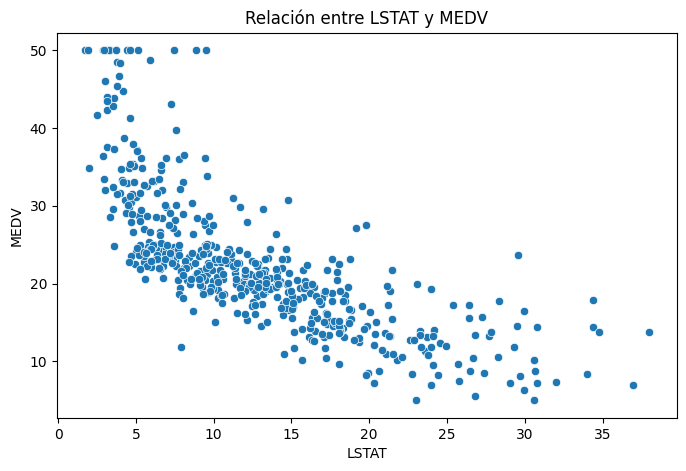
\includegraphics[width=\textwidth]{figures/lstat_medv.png}
    \caption{\footnotesize Porcentaje de población de bajo estatus}
    \label{fig:modelo_lstat}
\end{subfigure}

\caption{Distribución de variables por Valor Mediano de Viviendas}
\label{fig:distribucion_variables}
\end{figure}

Como podemos observar, todas las variables son significativas al momento de tomar en cuenta el precio de la casa. Por lo tanto, se utilizarán todas las variables para los diferentes modelos.

\vspace{0.5cm}

\subsection{Modelo lineal Gaussiano (MLG)}

Para realizar el MLG utilizamos el siguiente código:

\begin{lstlisting}[language=Python, frame=single, basicstyle=\ttfamily\small, breaklines=true]
splitter = ShuffleSplit(n_splits=50, test_size=0.3, random_state=42)

mae_scores_mlg, rmse_scores_mlg = [], []

for train_index, test_index in splitter.split(x):
    X_train, X_test = x[train_index], x[test_index]
    y_train, y_test = y[train_index], y[test_index]

    X_train_sm = sm.add_constant(X_train, has_constant='add')
    X_test_sm = sm.add_constant(X_test, has_constant='add')

    model_gaussian = sm.GLM(y_train, X_train_sm, family=sm.families.Gaussian())
    fitted = model_gaussian.fit()

    y_pred_gaussian = fitted.predict(X_test_sm)

    mae_scores_mlg.append(mean_absolute_error(y_test, y_pred_gaussian))
    rmse_scores_mlg.append(mean_squared_error(y_test, y_pred_gaussian) ** 0.5)


mae_median = np.median(mae_scores_mlg)
mae_std = np.std(mae_scores_mlg, ddof=1)
rmse_median = np.median(rmse_scores_mlg)
rmse_std = np.std(rmse_scores_mlg, ddof=1)

print(f"Gaussian Model – MAE: {mae_median:.2f} ± {mae_std:.2f}")
print(f"Gaussian Model – RMSE: {rmse_median:.2f} ± {rmse_std:.2f}")
\end{lstlisting}

Obteniendo los siguientes resultados:

\vspace{0.3cm}

\begin{table}[H]
\centering
\caption{Resultados del Modelo Lineal Gaussiano}\label{tab:regresion_resultados}
\begin{tabular}{lcc}
\toprule
\textbf{Métrica} & \textbf{Valor} \\
\midrule
MAE & 3.39 ± 0.22  \\
RMSE & 4.91 ± 0.45  \\
\bottomrule
\end{tabular}
\end{table}

\subsubsection{Interpretación de los resultados}

Los resultados del modelo lineal Gaussiano indica que la diferencia entre los valores reales de MEDV y los valores estimados por el modelo es de 3.39 mil dólares, con una variabilidad moderadamente baja.
El RMSE, al ser más sensible a errores grandes, indica que las desviaciones cuadráticas promedio equivalen a unos 4.91 mil dólares, lo que sugiere que existen algunos errores más grandes, aunque no dominantes.

\newpage

\subsection{K-Nearest Neighbors (KNN)}

Primero, definimos nuestras variables para poder trabajar con el modelo KNN.

\begin{lstlisting}[language=Python, frame=single, basicstyle=\ttfamily\small, breaklines=true]
x = muestra[['pregnancies', 'glucose', 'blood_pressure', 'skin_thickness',
'insulin', 'bmi', 'diabetes_pedigree', 'age']]
y = muestra['outcome']

X_train, X_test, y_train, y_test = train_test_split(x, y, random_state=4181, shuffle=True)
scaler = MinMaxScaler()
X_train = scaler.fit_transform(X_train)
X_test = scaler.transform(X_test)
\end{lstlisting}

Ahora, vamos a calcular el valor K que maximice la exactitud del modelo.

\begin{lstlisting}[language=Python, frame=single, basicstyle=\ttfamily\small, breaklines=true]
    k_range = range(1, 21)
scores = []
for k in k_range:
    knn = KNeighborsClassifier(n_neighbors=k)
    knn.fit(X_train, y_train)
    scores.append(knn.score(X_test, y_test))
plt.figure()
plt.xlabel('k')
plt.ylabel('Exactitud')
plt.scatter(k_range, scores)
plt.xticks([0, 5, 10, 15, 20])
plt.title('Exactitud vs. k en KNN')
plt.show()
\end{lstlisting}

Obteniendo la siguiente gráfica:

\begin{figure}[H]
\centering
\caption{Exactitud vs. k en KNN}
\label{fig:knn_accuracy}
\end{figure}

Por lo que decidimos utilizar el valor k=13 para nuestro modelo KNN.

\begin{lstlisting}[language=Python, frame=single, basicstyle=\ttfamily\small, breaklines=true]
knn = KNeighborsClassifier(n_neighbors=13)
knn.fit(X_train, y_train)
print("Exactitud en entrenamiento: {}".format(knn.score(X_train, y_train)))
print("Exactitud en prueba: {}".format(knn.score(X_test, y_test)))

y_pred = knn.predict(X_test)
y_pred_proba = knn.predict_proba(X_test)[:, 1]

precision = precision_score(y_test, y_pred)
sensibilidad = recall_score(y_test, y_pred)
f1 = f1_score(y_test, y_pred)
auc = roc_auc_score(y_test, y_pred)

print(f'Precision: {precision}')
print(f'Sensibilidad: {sensibilidad}')
print(f'F1 Score: {f1}')
print(f'AUC: {auc}')
\end{lstlisting}

Obteniendo los siguientes resultados:

\begin{table}[H]
\centering
\caption{Métricas de Rendimiento del Modelo KNN}\label{tab:knn_resultados}
\begin{tabular}{lc}
\toprule
\textbf{Métrica} & \textbf{Valor} \\
\midrule
Mejor valor de K & 13 \\
Exactitud en entrenamiento & 77.3\% \\
Exactitud en prueba & 72.8\% \\
Precisión (clase 1) & 52.8\% \\
Sensibilidad & 52.8\% \\
F1-Score & 52.8\% \\
AUC & 0.6683 \\
\bottomrule
\end{tabular}
\end{table}

\subsubsection{Interpretación de Resultados}
El modelo K-NN con k=13 demuestra un rendimiento moderado para la clasificación de diabetes, 
con una exactitud del 72.8\% en el conjunto de prueba. La diferencia entre la exactitud de 
entrenamiento (77.3\%) y prueba (72.8\%) sugiere un ligero sobreajuste, pero dentro de límites 
aceptables.

La precisión y sensibilidad idénticas del 52.8\% indican que el modelo mantiene un balance 
equilibrado entre la detección de verdaderos positivos y la minimización de falsos positivos. 
El valor de AUC de 0.668 muestra una capacidad discriminativa moderada, superior al azar pero 
con margen de mejora.

\vspace{1cm}

\subsection{Linear Discriminant Analysis (LDA)}

En la Linear Discriminant Analysis vamos a escalar nuevamente los datos antes de proceder: 

\begin{lstlisting}[language=Python, frame=single, basicstyle=\ttfamily\small, breaklines=true]
    x = muestra[['pregnancies', 'glucose', 'blood_pressure', 'skin_thickness',
'insulin', 'bmi', 'diabetes_pedigree', 'age']]
y = muestra['outcome']

x_train, x_test, y_train, y_test = train_test_split(x, y, test_size=0.2, random_state=4181, shuffle=True)

scaler = StandardScaler()
x_train_scaled = scaler.fit_transform(x_train)
x_test_scaled = scaler.transform(x_test)
\end{lstlisting}

Ahora, procedemos a realizar el modelo LDA:

\begin{lstlisting}[language=Python, frame=single, basicstyle=\ttfamily\small, breaklines=true]
    lda = LinearDiscriminantAnalysis()
    lda.fit(x_train_scaled, y_train)
    y_pred_lda = lda.predict(x_test_scaled)
\end{lstlisting}

Obteniendo los siguientes resultados:

\begin{table}[H]
\centering
\caption{Métricas de Rendimiento del Modelo Linear Discriminant Analysis}\label{tab:lda_resultados}
\begin{tabular}{lc}
\toprule
\textbf{Métrica} & \textbf{Valor} \\
\midrule
Exactitud en entrenamiento & 77.75\% \\
Exactitud en prueba & 75\% \\
Precisión (clase 1) & 61.29\% \\
Sensibilidad & 59.38\% \\
F1-Score & 60.32\% \\
AUC & 0.7086 \\
\bottomrule
\end{tabular}
\end{table}

\subsubsection{Interpretación de Resultados - Linear Discriminant Analysis}

El modelo LDA presenta un rendimiento sólido y equilibrado para la clasificación de diabetes, destacándose por su excelente capacidad de generalización con una diferencia mínima de 2.75 puntos porcentuales entre la exactitud de entrenamiento (77.75\%) y prueba (75\%), evidenciando prácticamente ausencia de sobreajuste. Con una precisión del 61.29\%, sensibilidad del 59.38\% y F1-Score del 60.32\%, LDA supera significativamente a KNN en todas las métricas (+8.5 puntos en precisión) y demuestra una capacidad discriminativa buena con un AUC de 0.7086, aproximándose al rendimiento de regresión logística (0.710). La estabilidad del modelo y su superior rendimiento en la minimización de falsos positivos lo posicionan como una opción robusta para la clasificación de diabetes, capturando efectivamente la estructura lineal de separación entre clases mientras mantiene un balance razonable entre precisión y sensibilidad.

\vspace{1cm}

\subsection{Quadratic Discriminant Analysis (QDA)}

Para realizar el Quadratic Discriminant Analysis utilizamos el siguiente código:

\begin{lstlisting}[language=Python, frame=single, basicstyle=\ttfamily\small, breaklines=true]
x = muestra[['pregnancies', 'glucose', 'blood_pressure', 'skin_thickness',
'insulin', 'bmi', 'diabetes_pedigree', 'age']]
y = muestra['outcome']

x_train, x_test, y_train, y_test = train_test_split(x, y, test_size=0.2, random_state=4181, shuffle=True)

scaler = StandardScaler()
x_train_scaled = scaler.fit_transform(x_train)
x_test_scaled = scaler.transform(x_test)

clf = QuadraticDiscriminantAnalysis()
clf.fit(x_train_scaled, y_train)

y_pred_qda = clf.predict(x_test_scaled)
\end{lstlisting}

Con este código obtenemos los siguientes resultados:

\begin{table}[H]
\centering
\caption{Métricas de Rendimiento del Modelo Quadratic Discriminant Analysis}\label{tab:qda_resultados}
\begin{tabular}{lc}
\toprule
\textbf{Métrica} & \textbf{Valor} \\
\midrule
Exactitud en entrenamiento & 77\% \\
Exactitud en prueba & 72\% \\
Precisión (clase 1) & 55.88\% \\
Sensibilidad & 59.38\% \\
F1-Score & 57.58\% \\
AUC & 0.6866 \\
\bottomrule
\end{tabular}
\end{table}

\subsubsection{Interpretación de Resultados - Quadratic Discriminant Analysis}

El modelo QDA presenta un rendimiento intermedio para la clasificación de diabetes, con una diferencia de 5 puntos porcentuales entre la exactitud de entrenamiento (77\%) y prueba (72\%), indicando un ligero sobreajuste superior al observado en LDA pero comparable con KNN. Con una precisión del 55.88\%, sensibilidad del 59.38\% y F1-Score del 57.58\%, QDA se posiciona entre KNN y LDA en términos de rendimiento general, superando a KNN (+3 puntos en precisión) pero siendo inferior a LDA (-5.4 puntos en precisión). Su capacidad discriminativa con un AUC de 0.6866 resulta intermedia, superior a KNN (0.668) pero inferior tanto a LDA (0.709) como a regresión logística (0.710), sugiriendo que la flexibilidad adicional de las fronteras cuadráticas no se traduce en una mejora significativa del rendimiento para este conjunto de datos específico, donde las relaciones parecen ser predominantemente lineales.

\newpage

\subsection{Naive Bayes Gaussiano}

Para realizar el Naive Bayes Gaussiano utilizamos el siguiente código: 

\begin{lstlisting}[language=Python, frame=single, basicstyle=\ttfamily\small, breaklines=true]
x = muestra[['pregnancies', 'glucose', 'blood_pressure', 'skin_thickness',
'insulin', 'bmi', 'diabetes_pedigree', 'age']]
y = muestra['outcome']

x_train, x_test, y_train, y_test = train_test_split(x, y, test_size=0.2, random_state=4181, shuffle=True)

scaler = StandardScaler()
x_train_scaled = scaler.fit_transform(x_train)
x_test_scaled = scaler.transform(x_test)

nb = GaussianNB()
nb.fit(x_train_scaled, y_train)

y_pred_nb = nb.predict(x_test_scaled)
\end{lstlisting}

Con este código obtenemos los siguientes resultados:

\begin{table}[H]
\centering
\caption{Métricas de Rendimiento del Modelo Naive Bayes Gaussiano}\label{tab:nb_resultados}
\begin{tabular}{lc}
\toprule
\textbf{Métrica} & \textbf{Valor} \\
\midrule
Exactitud en entrenamiento & 77\% \\
Exactitud en prueba & 79\% \\
Precisión (clase 1) & 65.71\% \\
Sensibilidad & 71.88\% \\
F1-Score & 68.66\% \\
AUC & 0.7711 \\
\bottomrule
\end{tabular}
\end{table}

\subsubsection{Interpretación de Resultados - Naive Bayes Gaussiano}

El modelo Naive Bayes Gaussiano presenta el mejor rendimiento general entre todos los modelos evaluados, destacándose por una situación excepcional donde la exactitud en prueba (79\%) supera a la de entrenamiento (77\%), indicando una excelente capacidad de generalización sin sobreajuste. Con la mayor sensibilidad (71.88\%) de todos los modelos, Naive Bayes demuestra superior capacidad para detectar casos reales de diabetes, lo cual es crítico en aplicaciones médicas donde no identificar un caso positivo puede tener consecuencias graves. Su precisión del 65.71\% es la más alta obtenida, minimizando efectivamente los falsos positivos, mientras que el F1-Score de 68.66\% refleja el mejor balance entre precisión y sensibilidad. El AUC de 0.7711 confirma la mejor capacidad discriminativa entre todas las técnicas evaluadas, superando incluso a la regresión logística (0.710) y LDA (0.709). Estos resultados sugieren que el supuesto de independencia condicional del algoritmo, aunque teóricamente restrictivo, funciona efectivamente en este conjunto de datos específico, posicionando a Naive Bayes como la opción más robusta para la clasificación de diabetes en términos de rendimiento predictivo y estabilidad del modelo.

\newpage

\subsection{10-fold Cross-Validation}

Para realizar nuestro Cross-Validation utilizamos el siguiente código:

\begin{lstlisting}[language=Python, frame=single, basicstyle=\ttfamily\small, breaklines=true]
    x = muestra[['pregnancies', 'glucose', 'blood_pressure', 'skin_thickness',
            'insulin', 'bmi', 'diabetes_pedigree', 'age']]
    y = muestra['outcome']

    cv = StratifiedKFold(n_splits=10, shuffle=True, random_state=4181)  

    scoring = ['accuracy', 'precision', 'recall', 'f1', 'roc_auc']

    scaler = StandardScaler()
    x_scaled = scaler.fit_transform(x)

    #logistic Regression Cross Validation
    logistic = LogisticRegression(penalty=None)
    lr_results = cross_validate(logistic, x_scaled, y, cv=cv, scoring=scoring)

    #K-Nearest Neighboor Cross Validation]
    scaler_knn = MinMaxScaler()
    x_scaled_knn = scaler_knn.fit_transform(x)
    knn = KNeighborsClassifier(n_neighbors=13)
    knn_results = cross_validate(knn, x_scaled, y, cv=cv, scoring=scoring)

    #Linear Discriminant Analysys (LDA) Cross Validation

    lda = LinearDiscriminantAnalysis()
    lda_results = cross_validate(lda, x_scaled, y, cv=cv, scoring=scoring)  

    #Quadratic Discriminant Analysis (QDA) Cross Validation
    clf = QuadraticDiscriminantAnalysis()
    qda_results = cross_validate(clf, x_scaled, y, cv=cv, scoring=scoring)  

    #Naive Bayes Gaussiano Cross Validation
    nb = GaussianNB()
    nb_results = cross_validate(nb, x_scaled, y, cv=cv, scoring=scoring)    
\end{lstlisting}

\newpage

Obteniendo los siguientes resultados:

\begin{table}[H]
\centering
\caption{Resultados de Validación Cruzada 10-Fold}\label{tab:cross_validation}
\footnotesize
\begin{tabular}{lccccc}
\toprule
\textbf{Modelo} & \textbf{Exactitud} & \textbf{Precisión} & \textbf{Sensibilidad} & \textbf{F1-Score} & \textbf{AUC} \\
\midrule
Reg. Logística & 0.766±0.081 & 0.713±0.131 & 0.544±0.186 & 0.605±0.149 & 0.826±0.087 \\
KNN (k=13) & 0.748±0.059 & 0.676±0.093 & 0.514±0.158 & 0.575±0.123 & 0.782±0.093 \\
LDA & 0.762±0.090 & 0.705±0.147 & 0.538±0.199 & 0.597±0.161 & 0.823±0.092 \\
QDA & 0.744±0.107 & 0.659±0.162 & 0.538±0.195 & 0.584±0.176 & 0.798±0.097 \\
Naive Bayes & 0.768±0.093 & 0.687±0.142 & 0.613±0.186 & 0.639±0.148 & 0.809±0.098 \\
\bottomrule
\end{tabular}
\end{table}

\subsubsection{Interpretación de Resultados - 10-fold Cross-Validation}

La validación cruzada revela que, para las diferentes medidas, existen diferentes modelos que se desempeñan mejor.

\begin{itemize}
\item Exactitud: El modelo de Naive Bayes Gaussiano tiene la mayor exactitud promedio.
\item Precisión: La regresión logística tiene la mayor precisión promedio.
\item Sensibilidad: El Naive Bayes Gaussiano tiene la mayor sensibilidad promedio.
\item F1-Score: El Naive Bayes Gaussiano tiene el mayor F
\item AUC: La regresión logística tiene el mayor AUC promedio.
\end{itemize}

\subsection{Discusión de Resultados}

\subsubsection{Contexto Médico y Relevancia Clínica}

El dataset Pima Indians Diabetes presenta características particulares que influyen significativamente en la interpretación de los resultados obtenidos. Las mujeres de la tribu Pima tienen una de las tasas más altas de diabetes tipo 2 a nivel mundial, con una prevalencia que puede superar el 50\% en adultos, lo que convierte a esta población en un caso de estudio crítico para la predicción temprana de la enfermedad.

\subsubsection{Análisis Comparativo de Modelos}

Los resultados de validación cruzada revelan diferencias importantes entre los modelos evaluados, cada uno con implicaciones clínicas específicas:

\vspace{0.5cm}

\textbf{Regresión Logística: El Estándar Clínico}

La regresión logística demostró ser el modelo más robusto en términos de capacidad discriminativa (AUC = 0.826) y precisión (0.713), características fundamentales en el contexto médico. Su alta precisión minimiza los falsos positivos, reduciendo la ansiedad innecesaria en pacientes y los costos asociados con pruebas adicionales. El AUC superior indica una excelente capacidad para distinguir entre pacientes con y sin diabetes, lo cual es crítico para la toma de decisiones clínicas informadas.

\newpage

\textbf{Naive Bayes: Máxima Sensibilidad Clínica}

El modelo Naive Bayes Gaussiano sobresale por su sensibilidad superior (0.613), característica crucial en medicina preventiva donde el costo de no detectar un caso de diabetes (falso negativo) puede ser devastador para la salud del paciente. En el contexto de la tribu Pima, donde la diabetes puede progresar rápidamente y causar complicaciones graves, maximizar la detección temprana es prioritario sobre minimizar los falsos positivos.

\vspace{0.5cm}

\textbf{Implicaciones de los Modelos Lineales (LDA vs QDA)}

La superioridad de LDA sobre QDA (AUC: 0.823 vs 0.798) sugiere que las relaciones entre las variables predictoras y el riesgo de diabetes en esta población son predominantemente lineales. Este hallazgo tiene implicaciones importantes para el entendimiento de la patofisiología de la diabetes en la población Pima, indicando que los factores de riesgo actúan de manera aditiva rather than interactive.

\subsubsection{Consideraciones Específicas del Contexto Pima}

\textbf{Factores Genéticos y Ambientales}

Los resultados confirman la importancia de factores modificables como el BMI y la glucosa, pero también revelan la influencia significativa de variables como pregnancies y diabetes pedigree, que reflejan tanto factores genéticos como ambientales específicos de esta población. La alta prevalencia de diabetes gestacional en las mujeres Pima se refleja en la importancia predictiva del número de embarazos.

\subsubsection{Recomendaciones Clínicas Basadas en los Resultados}

\begin{itemize}
\item \textbf{Screening Primario:} Utilizar Naive Bayes para maximizar la detección temprana en programas de screening poblacional
\item \textbf{Confirmación Diagnóstica:} Emplear regresión logística cuando se requiera alta especificidad para confirmar casos sospechosos
\item \textbf{Monitoreo Continuo:} Implementar LDA para seguimiento longitudinal de pacientes de riesgo, aprovechando su estabilidad y interpretabilidad
\end{itemize}

\subsection{Matriz de Confusión}

\begin{figure}[H]
    \centering
    \caption{\footnotesize Embarazos}
    \label{fig:matriz_confusion}
\end{figure}

Según la Matriz de Confusión, podemos interpretar los resultados como: 

\begin{itemize}
\item 79 de 100 casos positivos fueron correctamente identificados (Verdaderos Positivos).
\item 12 falsos positivos fueron identificados, lo que indica que 12 personas sin diabetes fueron clasificadas erróneamente como diabéticas.
\item 9 falsos negativos, lo que significa que 9 personas con diabetes no fueron detectadas por el modelo.
\end{itemize}

\subsection{Conclusión}

En el contexto específico de la población Pima Indians, donde la diabetes representa una crisis de salud pública, los modelos desarrollados ofrecen herramientas valiosas para la detección temprana y prevención. La elección del modelo óptimo debe basarse en el objetivo clínico específico: Naive Bayes para screening poblacional donde la sensibilidad es prioritaria, y regresión logística para confirmación diagnóstica donde la especificidad es crucial. La implementación exitosa de estos modelos requiere integración cuidadosa con el contexto cultural y los recursos de salud disponibles en la comunidad.



\section{Ejercicio 2: California Housing}

Se trabajará con el dataset California Housing, que contiene información sobre viviendas en California.
El objetivo es predecir el valor mediano de las viviendas (variable objetivo continua, en unidades de
100,000 dólares).

\vspace{0.5cm}

Variables predictoras:
\begin{itemize}
\item MedInc: Ingreso mediano del hogar (en decenas de miles de dólares)
\item HouseAge: Edad mediana de las viviendas (en años)
\item AveRooms: Número promedio de habitaciones por vivienda
\item AveBedrms: Número promedio de dormitorios por vivienda
\item Population: Población del bloque
\item AveOccup: Ocupación promedio de las viviendas
\item Latitude: Latitud del bloque
\item Longitude: Longitud del bloque
\end{itemize}

Para exportar los datos utilizamos el siguiente código:

\begin{lstlisting}[language=Python, frame=single, basicstyle=\ttfamily\small, breaklines=true]
from sklearn.datasets import fetch_california_housing
california = fetch_california_housing()
X = california.data
y = california.target
\end{lstlisting}

\subsubsection{Búsqueda de Hiperparámetros con Grid Search:}
Realizamos grid search con validación cruzada de 5 folds para encontrar los mejores hiperparámetros para los tres modelos:

\begin{lstlisting}[language=Python, frame=single, basicstyle=\ttfamily\small, breaklines=true]
cv = KFold(n_splits=5, shuffle=True, random_state=4181)
\end{lstlisting}

\vspace{0.5cm}

\textbf{Lasso Regression:}

\begin{lstlisting}[language=Python, frame=single, basicstyle=\ttfamily\small, breaklines=true]
lasso_params = {
    'alpha': np.logspace(-4, 2, 20)
}
lasso = Lasso(random_state=42, max_iter=10000)
lasso_grid = GridSearchCV(
    estimator=lasso,
    param_grid=lasso_params,
    cv=cv,
    scoring='neg_mean_squared_error',
    n_jobs=-1,
    verbose=1
)

lasso_grid.fit(X_train_scaled, y_train)
\end{lstlisting}

\textbf{Ridge Regression:}
\begin{lstlisting}[language=Python, frame=single, basicstyle=\ttfamily\small, breaklines=true]
ridge_params = {
    'alpha': np.logspace(-4, 2, 20)
}
ridge = Ridge(random_state=42)
ridge_grid = GridSearchCV(
    estimator=ridge,
    param_grid=ridge_params,
    cv=cv,
    scoring='neg_mean_squared_error',
    n_jobs=-1,
    verbose=1
)
ridge_grid.fit(X_train_scaled, y_train)
\end{lstlisting}

\vspace{0.5cm}

\textbf{Elastic Net:}
\begin{lstlisting}[language=Python, frame=single, basicstyle=\ttfamily\small, breaklines=true]
elastic_params = {
    'alpha': np.logspace(-4, 2, 10),
    'l1_ratio': np.linspace(0, 1, 10)
}

elastic = ElasticNet(random_state=42, max_iter=10000)
elastic_grid = GridSearchCV(
    estimator=elastic,
    param_grid=elastic_params,
    cv=cv,
    scoring='neg_mean_squared_error',
    n_jobs=-1,
    verbose=1
)
elastic_grid.fit(X_train_scaled, y_train)
\end{lstlisting}

\subsubsection{Evaluación y Comparación de Modelo:}
Para cada modelo, con sus mejores hiperparámetros encontramods evaluaremos usando cross validation de 5 folds en el conjunto de entrenamiento:

\vspace{0.5cm}

\begin{lstlisting}[language=Python, frame=single, basicstyle=\ttfamily\small, breaklines=true]
lasso_validation = cross_val_score(lasso_grid.best_estimator_, X_test_scaled, y_test, cv=5, scoring='neg_mean_squared_error')
ridge_validation = cross_val_score(ridge_grid.best_estimator_, X_test_scaled, y_test, cv=5, scoring='neg_mean_squared_error')
elastic_validation = cross_val_score(elastic_grid.best_estimator_, X_test_scaled, y_test, cv=5, scoring='neg_mean_squared_error')
\end{lstlisting}

\newpage

Dándonos como resultado: 

\begin{table}[H]
\centering
\caption{Resultados de Validación Cruzada 5-Fold}\label{tab:cross_validation_LRE}
\footnotesize
\begin{tabular}{lc}
\toprule
\textbf{Modelo} & \textbf{CV Score}\\
\midrule
Lasso & 0.5028 (+/- 0.1239) \\
Ridge & 0.5114 (+/- 0.1317) \\
ElasticNet & 0.5026 (+/- 0.1225) \\
\bottomrule
\end{tabular}
\end{table}

\vspace{0.5cm}

Ahora, vamos a calcular Root Mean Square Error y Mean Absolute Error para cada modelo:

\begin{lstlisting}[language=Python, frame=single, basicstyle=\ttfamily\small, breaklines=true]
best_lasso = lasso_grid.best_estimator_
best_ridge = ridge_grid.best_estimator_
best_elastic = elastic_grid.best_estimator_

y_pred_lasso = best_lasso.predict(X_test_scaled)
y_pred_ridge = best_ridge.predict(X_test_scaled)
y_pred_elastic = best_elastic.predict(X_test_scaled)
\end{lstlisting}

\begin{table}[H]
\centering
\caption{Resultados de RMSE y MAE}\label{tab:RMSE_MAE}
\footnotesize
\begin{tabular}{lcc}
\toprule
\textbf{Modelo} & \textbf{RMSE} & \textbf{MAE}\\
\midrule
Lasso & 0.7427 & 0.5365\\
Ridge & 0.7433 & 0.5360\\
ElasticNet & 0.7426 & 0.5366\\
\bottomrule
\end{tabular}
\end{table}

\subsubsection{Análisis de Resultados}

\vspace{0.5cm}

\textbf{Lasso:}

\vspace{0.3cm}

\textbf{¿Cuántas variables tienen coeficientes exactamente iguales a cero?}

El modelo Lasso tiene 1 variable con coeficiente exactamente igual a cero.

\vspace{0.3cm}

\textbf{¿Qué variables fueron eliminadas del modelo?}

La variable eliminada por Lasso es Population.

\vspace{0.5cm}

\textbf{Ridge:}

\vspace{0.3cm}

\textbf{¿Cuántas variables tienen coeficientes cercanos a cero (|coeficiente|<0,01)?}

Tenemos 1 variable con coeficiente cercano a cero.

\vspace{0.3cm}

\textbf{¿Cómo se comparan las magnitudes de los coeficientes con los de Lasso?}

Al sumar el total de los valores absolutos tenemos: 

\begin{itemize}
\item Lasso: 3.2259
\item Ridge: 3.3015
\end{itemize}

También, viendo los comportamientos por variables obtenemos: 

\begin{table}[H]
\centering
\caption{Comparativa por Variable}\label{tab:comparativa_por_variable}
\footnotesize
\begin{tabular}{lcc}
\toprule
\textbf{Variable} & \textbf{Lasso} & \textbf{Ridge}\\
\midrule
MedInc & 0.8295 & 0.8382\\
HouseAge & 0.1249 & 0.1248\\
AveRooms & -0.2408 & -0.2612\\
AveBedrms & 0.2839 & 0.3039\\
Population & -0.0000 & -0.0004\\
AveOccup & -0.0379 & -0.0397\\
Latitude & -0.8686 & -0.8803\\
Longitude & -0.8403 & -0.8530\\
\bottomrule
\end{tabular}
\end{table}

Ridge mantiene todas las variables en el modelo con coeficientes ligeramente superiores en magnitud (suma total de 3.3015 vs 3.2259 de Lasso), aplicando una penalización uniforme que reduce pero no elimina completamente ninguna variable. En contraste, Lasso demuestra su capacidad de selección automática de características al eliminar completamente la variable Population, asignándole un coeficiente de exactamente cero, mientras que Ridge la conserva con un valor mínimo de -0.0004. Las diferencias más pronunciadas se observan en AveRooms y AveBedrms, donde Ridge presenta coeficientes 8.48% y 7.04% superiores respectivamente, sugiriendo que la regularización L2 de Ridge distribuye la penalización más uniformemente entre todas las variables correlacionadas.

\vspace{0.5cm}

\textbf{Elastic Net:}

\vspace{0.3cm}

\textbf{Basado en el mejor valor de l1 ratio encontrado, ¿el modelo se comporta más como Lasso o como
Ridge?}

El modelo se comporta más como Lasso.

\vspace{0.3cm}

\textbf{¿Qué ventajas ofrece Elastic Net sobre los otros dos métodos en este dataset?}

En este caso particular, Elastic Net no ofrece ventajas significativas sobre Lasso y Ridge debido a que converge a un comportamiento idéntico al de Lasso puro (l1\_ratio = 1.0). Esto significa que el algoritmo de optimización determinó que la regularización L1 pura era la más efectiva para este dataset, eliminando completamente el componente L2. Sin embargo, las ventajas teóricas de Elastic Net incluyen: 

\begin{itemize}
\item Estabilidad en selección de variables: cuando existen grupos de variables altamente correlacionadas, Elastic Net tiende a seleccionar grupos completos en lugar de elegir arbitrariamente una variable del grupo como hace Lasso.
\item Flexibilidad en regularización: permite encontrar el balance óptimo entre selección de características (L1) y reducción uniforme de coeficientes (L2) mediante el parámetro l1\_ratio.
\item Robustez numérica: es menos sensible a pequeños cambios en los datos comparado con Lasso puro, especialmente cuando n < p (más variables que observaciones). 
\end{itemize}

No obstante, en el dataset California Housing, la ausencia de multicolinealidad severa y la naturaleza de las variables explicativas hicieron que Lasso fuera suficiente, por lo que Elastic Net no proporcionó beneficios adicionales, convergiendo naturalmente hacia la regularización L1 pura y produciendo resultados prácticamente idénticos a Lasso tanto en coeficientes como en métricas de rendimiento (RMSE: 0.7426 vs 0.7427).

\subsubsection{Conclusión}

Según el Cuadro 9: Resultados de RMSE y MAE, podemos presentar que el mejor modelo es Elastic Net debido a:

\begin{itemize}
    \item Tiene el menor RMSE (0.7426) lo que indica mejor capacidad predictiva
    \item Las diferencias entre los tres modelos son muy pequeñas
    \item Converge a Lasso puro, pero el proceso de optimización le permite encontrar una solución ligeramente superior.
    \item Ofrece mayor estabilidad numérica en el proceso de Optimización
    \item Elimina automáticamente variables irrelevantes al igual que Lasso.
\end{itemize}

En términos prácticos, los tres modelos tienen rendimientos idénticos, pero Elastic Net logra la mejor combinación de presición predictiva y selección automática de características, posicionándolo como la opción óptima para este dataset.

\section{Referencias}

\begin{thebibliography}{9}

\bibitem{regresion_logistica}
Ciencia de Datos. \textit{Regresión Logística con Python}. 
\url{https://cienciadedatos.net/documentos/py17-regresion-logistica-python}

\bibitem{knn_tutorial}
Aprende Machine Learning. \textit{Clasificar con K-Nearest Neighbor: Ejemplo en Python}. 
\url{https://www.aprendemachinelearning.com/clasificar-con-k-nearest-neighbor-ejemplo-en-python/}

\bibitem{lda_geeks}
GeeksforGeeks. \textit{Linear Discriminant Analysis in Machine Learning}. 
\url{https://www.geeksforgeeks.org/machine-learning/ml-linear-discriminant-analysis/}

\bibitem{qda_sklearn}
Scikit-learn Documentation. \textit{QuadraticDiscriminantAnalysis}. 
\url{https://scikit-learn.org/stable/modules/generated/sklearn.discriminant_analysis.QuadraticDiscriminantAnalysis.html}

\bibitem{naive_bayes}
GeeksforGeeks. \textit{Gaussian Naive Bayes}. 
\url{https://www.geeksforgeeks.org/machine-learning/gaussian-naive-bayes/}

\bibitem{cross_validation}
GeeksforGeeks. \textit{Cross Validation using K-Fold with Scikit Learn}. 
\url{https://www.geeksforgeeks.org/machine-learning/cross-validation-using-k-fold-with-scikit-learn/}

\bibitem{mae_python}
GeeksforGeeks. \textit{How to Calculate Mean Absolute Error in Python}. 
\url{https://www-geeksforgeeks-org.translate.goog/python/how-to-calculate-mean-absolute-error-in-python/}

\end{thebibliography}

\end{document}
